\section*{Speed of light}
In order to measure the speed of light , the $\gamma$ source was moved between the two detectors. The position of the source~($x$) with respect to the detectors was considered as shown in Fig.~\ref{Fig:Src_pos}.
\begin{figure}[h!]
	\centering
	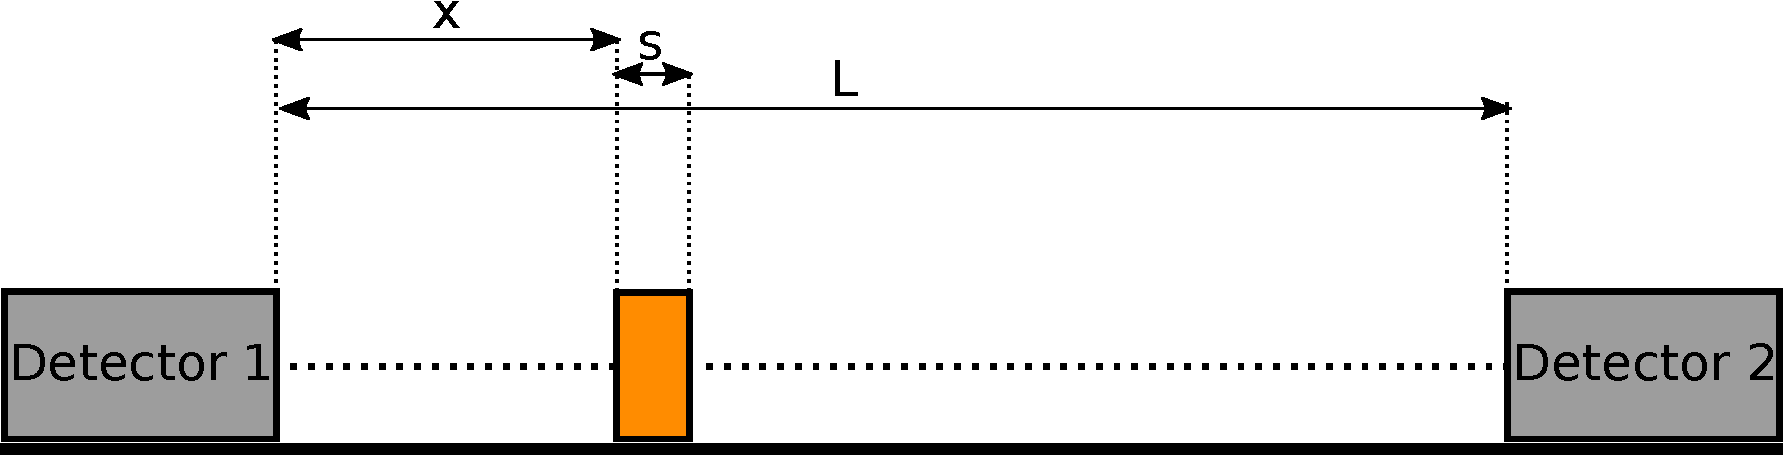
\includegraphics[width=0.8\textwidth]{Light_Speed_setup}
	\caption{Source position between the detectors.}
	\label{Fig:Src_pos}
\end{figure}

Considering the two coincident $\gamma$ emission at $t=0$ the signals produced by the detectors will have the following timing reference:

\[
\begin{aligned}
T_1 &=\frac{x+s/2}{c}+\delta_1\\
T_2 &=\frac{L-x-s/2}{c}+\delta_2
\end{aligned}
\]

where $\delta_1$ and $\delta_2$ are the constant cable delays of the electronic setup.  Therefore the TAC will shows the time value:

\[
T_{\text{TAC}}=T_1-T_2=\frac{2 x}{c}+const.
\] 

Using four different $x$ positions the  TAC distribution of Fig.~\ref{Fig:TAC_speed_dist} were produced.

\begin{figure}[h]
	\centering
	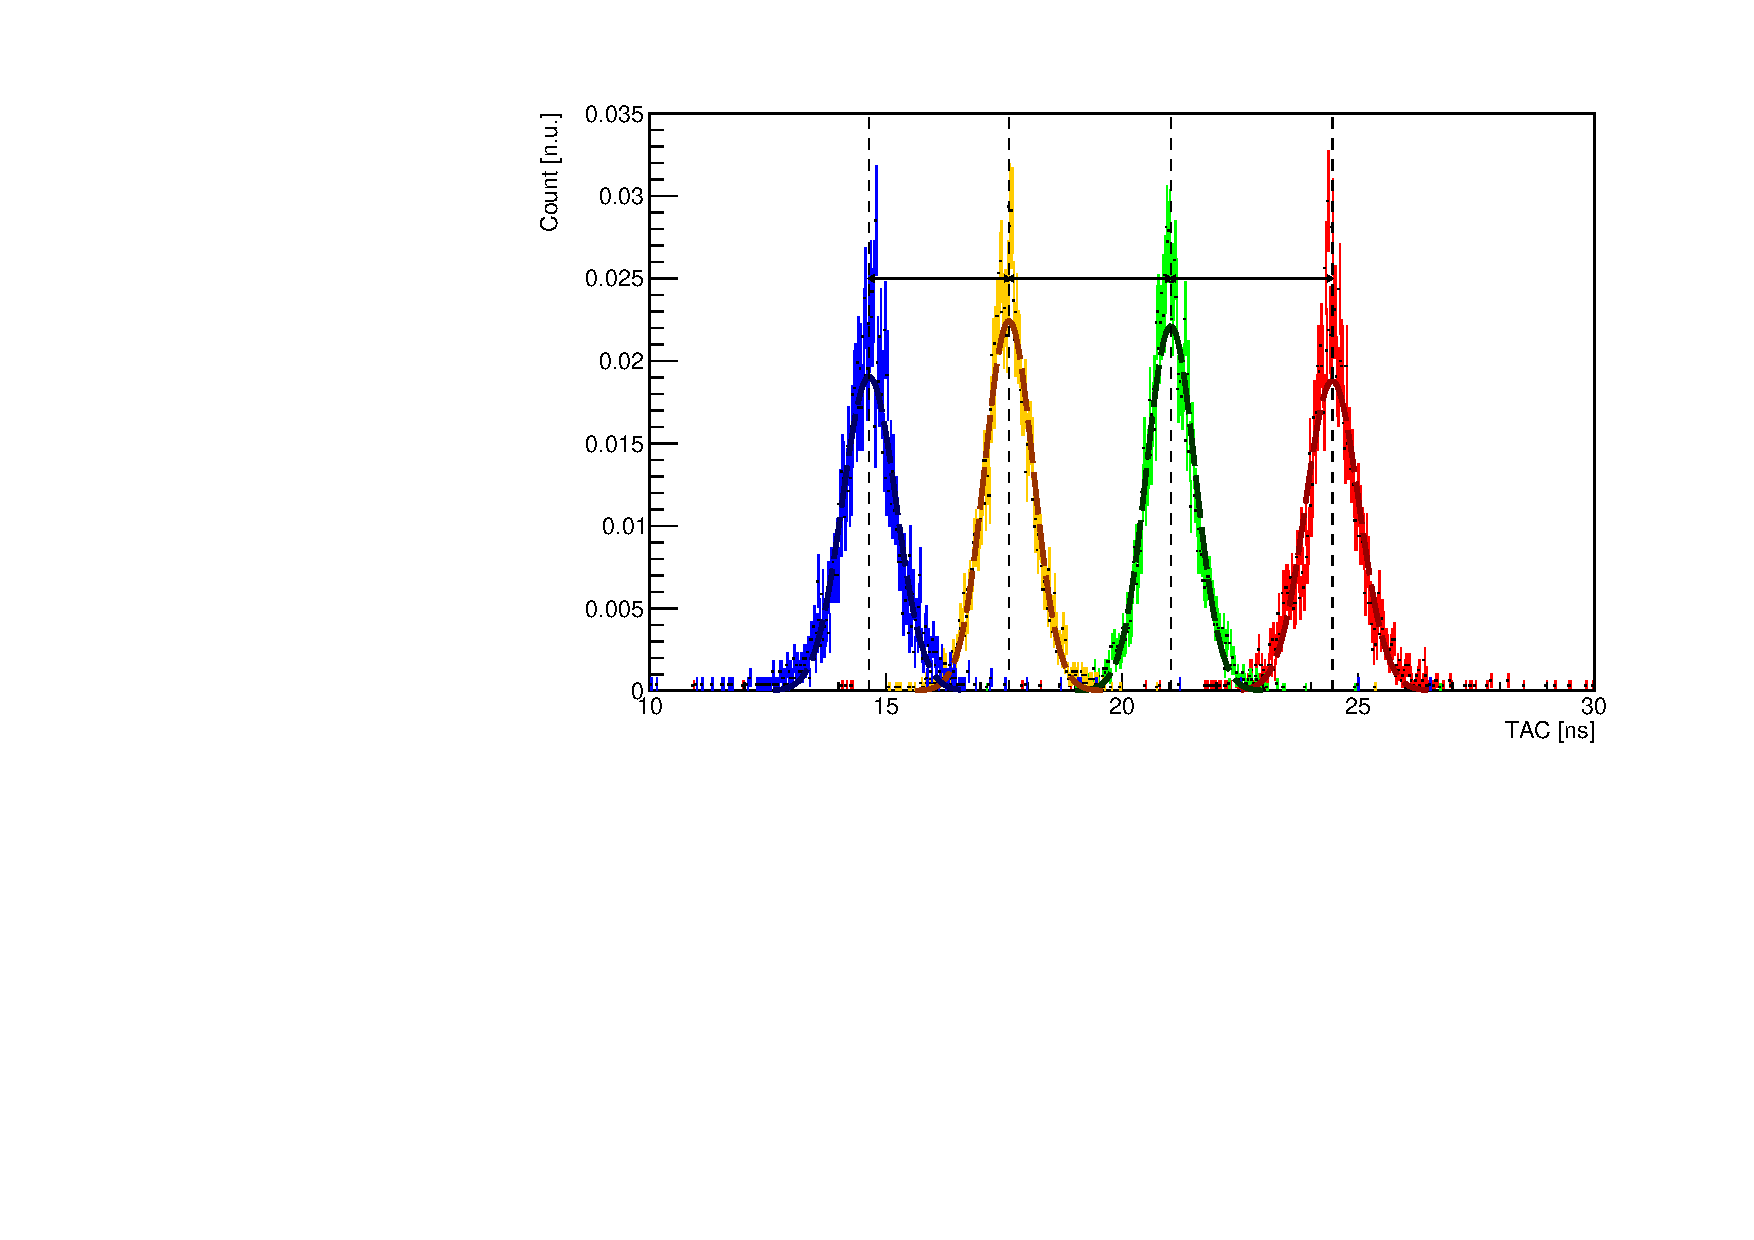
\includegraphics[width=0.8\textwidth]{TACoverlayed_dist}
	\caption{TAC distribution obtained in the four different $x$ positions.}
	\label{Fig:TAC_speed_dist}
\end{figure}

Computing the centroids of the peaks it was possible to draw $x$ as a function of $T_{\text{TAC}}$ as shown in Fig.~\ref{Fig:Speed_fit} and perform a linear fit where the angular coefficient corresponds to $c/2$.
 
 \begin{figure}[H]
 	\begin{minipage}[b]{0.6\textwidth}
\centering
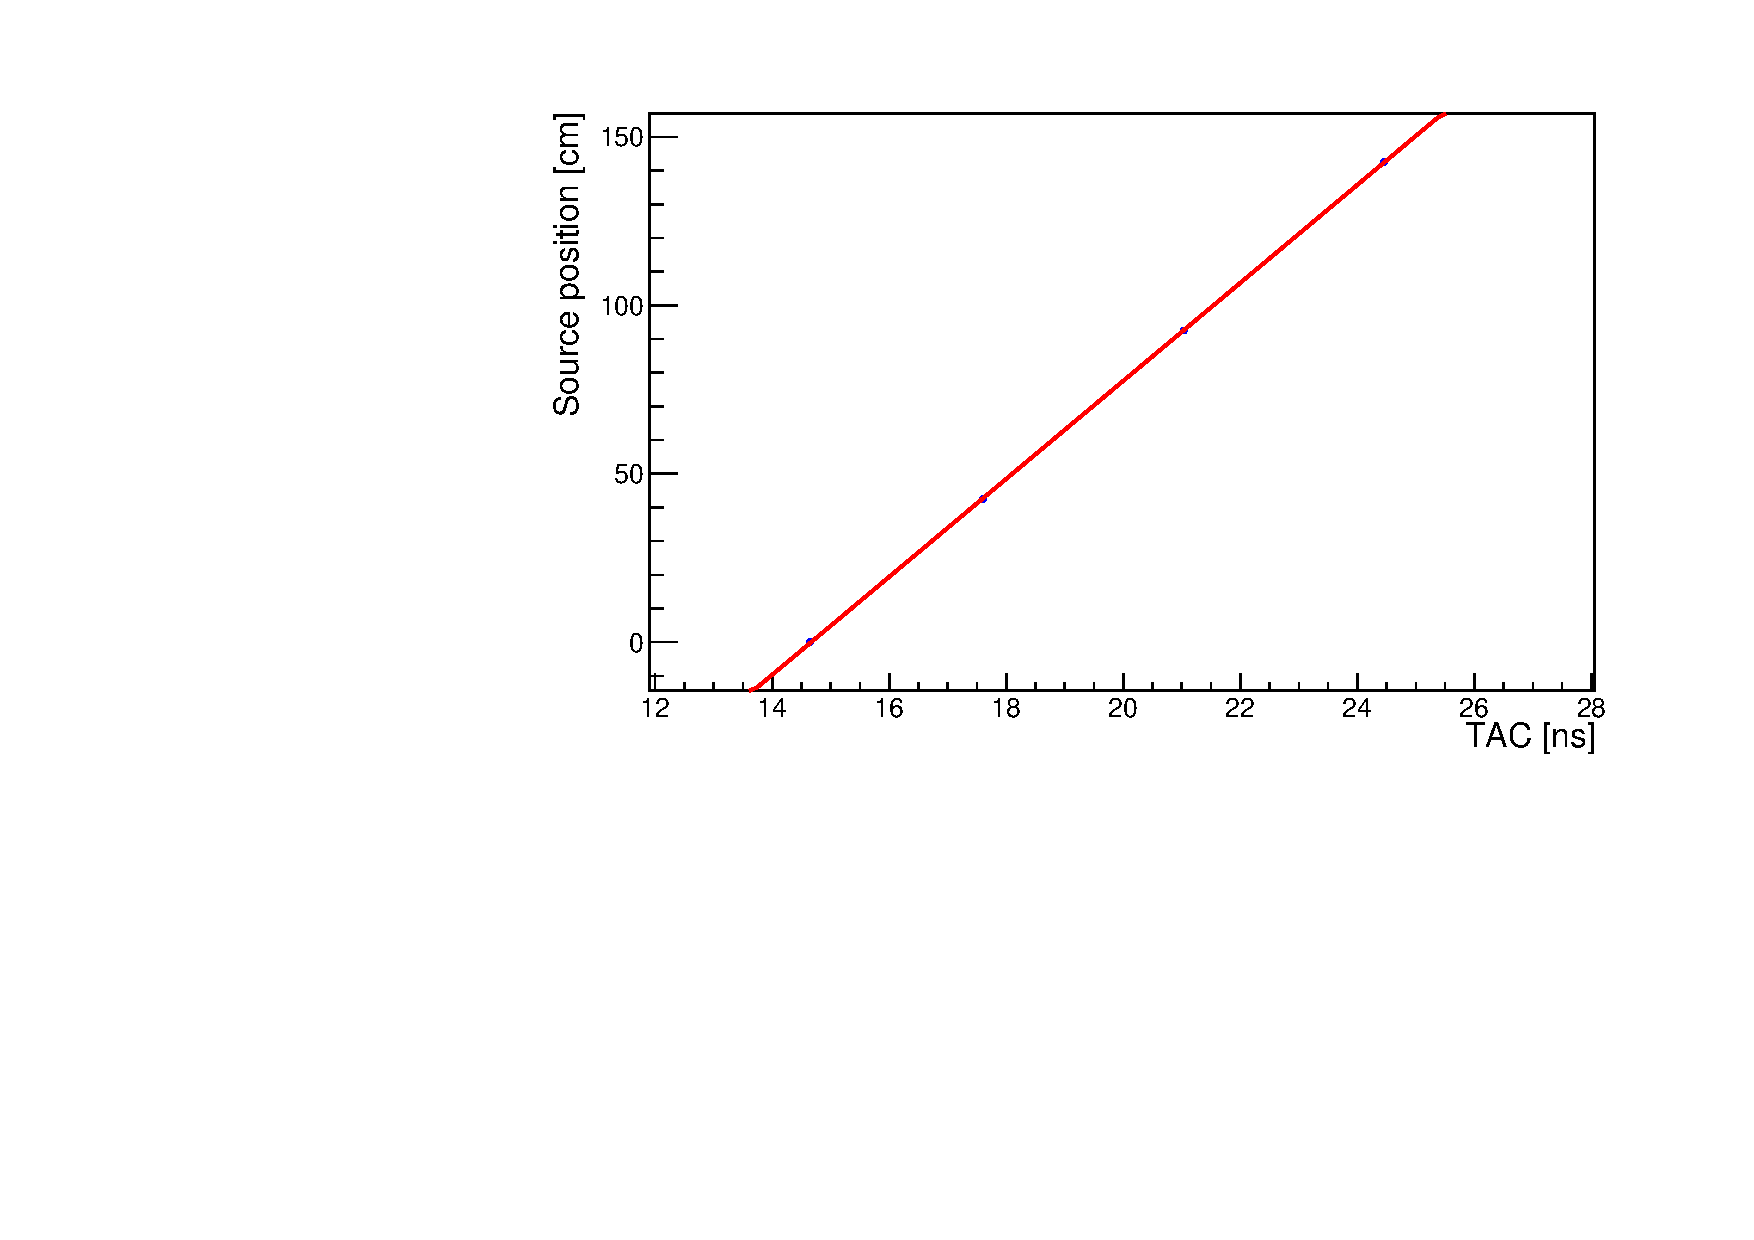
\includegraphics[width=\textwidth]{Speed_fit}
\caption{Linear Fit of $x$ position as a function of $T_{\text{TAC}}$ .}
\label{Fig:Speed_fit}
 	\end{minipage}
 	\hfill
 	\begin{minipage}[b]{0.45\textwidth}
 		\centering
 		\begin{tabular}{cc}
 			\toprule
 			\toprule
 			Parameter & Value \\
 			\midrule
 			p0     & ( -2.133$\pm$0.006)$\times 10^2$~cm \\
 			p1     & 14.54$\pm$0.03~cm/ns\\
 			c        & 29.08 $\pm$0.06~cm/ns\\
 			\bottomrule
 			\bottomrule
 		\end{tabular}
 		\vspace{1.45cm}
 		\caption*{Fit parameters and computed speed of light.}
 	\end{minipage}
 \end{figure}

